% Skrivet av Erik

%\todo{Förklara övergripande struktur och syfte för NewSegSiev och underordnade funktioner, ev. med en flowchart.} 
%Algoritmen genererar alla primtal (till kvadraten av det sista primtalet vi sållar med) och kan enkelt utföras med papper och penna, men hur kan algoritmen förbättras för dagens datororienterade algoritmer? 

% Typ:
%Vi vill sålla fram primtal ur ett intervall. Vi gör detta genom eratosthones såll. Börjar med alla tal i intervallet och sedan stryker vi sånt som är multiplar av tal mindre än sqrt(övregränsen) Vi delar in dessa tal i två kategorier
%1. Små tal, dessa är så små att de alltid har multiplar i intervallet. Vi sållar precis som Erat. för dessa. 
%2. Större tal, här är det inte säkert att det har en multipel i intervallet och vi kan börjar med en uppskattning var att se om så är fallet

När Eratosthenes först formulerade sitt såll var det, som vi såg i inledningen, på formen av en algoritm. Det är med utgångspunkt i Eratosthenes ursprungliga idé som \cite{HaraldSieve} utvecklar algoritmen för att optimera processen till en effektiv kod som kan leta efter primtal i ett intervall, $[n - \Delta, n + \Delta] \subset \mathbb{R}_+$. Delvis gör \cite{HaraldSieve} detta med en algoritm som han kallar \textsc{SimpleSiev}, vilken är nära en direkt översättning av Eratosthenes klassiska såll, för att erhålla en lista av alla primtal upp till ett givet tal $N$. Denna metoden fungerar väl för små $N$ men vill vi hitta primtal i ett intervall $[n - \Delta, n + \Delta]$ för något stort $n$ och litet $\Delta$ så ger algoritmen oss betydligt mer information än vad vi behöver och kräver mer tid och minnesutrymme. 

Flaggskeppet i \cite{HaraldSieve}, algoritmen \textsc{NewSegSiev}, löser problemet genom att dela upp talen vi vill sålla bort multiplar av i två fall --- tal som är så pass små att vi är garanterade att det finns en multipel av dessa i vårt intervall och större tal som vi inte kan lika säkra på. Med den här uppdelningen kan vi behandla de båda fallen olika för att spara tid och precis som i Eratosthenes såll behöver vi inte sålla med tal större än \(\sqrt{n + \Delta}\). 

Eftersom vi kan vara säkra på att alla tal mindre än längden av intervallet (det vill säga \(m \leq 2 \Delta\)) har en multipel i intervallet så börjar vi att sålla för dessa. \todo{nämna marginalen K Delta} Processen i \textsc{NewSegSiev} för \(m \leq K \Delta\) är i sin tur delad i tre funktioner

Vi behöver som bekant inte sålla för alla tal utan det räcker med att vi utesluter multiplar av primtal så vi

\textsc{NewSegSiev} gör detta genom att först kalla på en funktion \textsc{SubSegSiev} vilken sållar för mindre primtal och använder en segmenterad variant av Eratosthenes såll. För större primtal utnyttjar Helfgott en del analytiska metoder för att effektivisera sökandet efter multiplar i intervallet. Vi börjar med att kolla på strukturen av \textsc{SubSegSiev} före vi sedan studerar Helfgotts matematiska resonemang för \textsc{NewSegSiev}:s pseudokod.

\begin{figure}
    \centering
    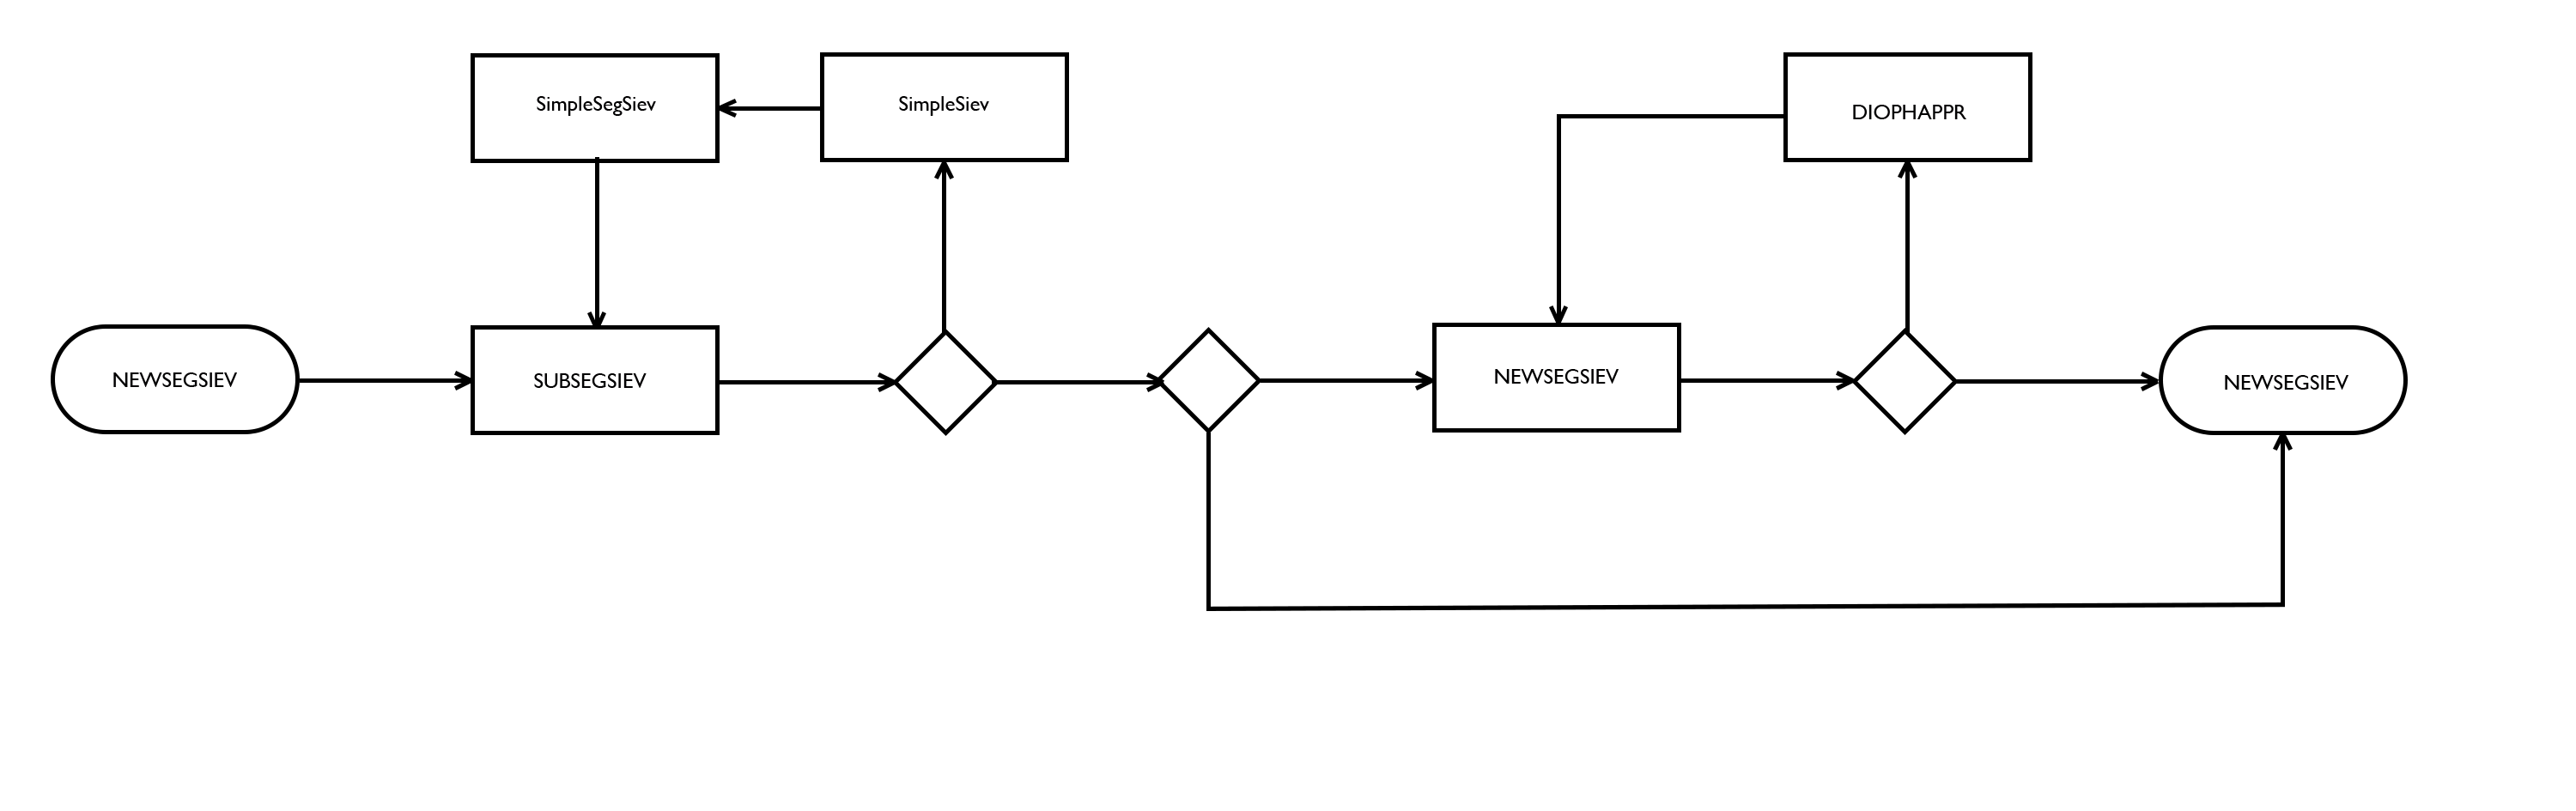
\includegraphics[width = \textwidth]{erik/Images/flowchart.png}
    \caption{Placeholder}
    \label{fig:flowchart}
\end{figure}

Målet med \textsc{SubSegSiev} är att, givet \(n, \Delta \) och $M$, sålla \([n, n + \Delta]\) med primtal $p \leq M$. Algoritmen gör detta på i stort sett samma vis som i Eratosthenes klassiska såll men delar in primtalen i segment för att optimera minneskomplexiteten. \todo{Fortsätt med att gå igenom SimpleSiev, SimpleSegSiev och SubSegSiev och kort förklara hur de samverkar i NewSegSiev}.

Nästa steg, algoritmen i \textsc{NewSegSiev}, kräver mer matematisk eftertanke. Uppgiften som kvarstår för funktionen efter \textsc{SubSegSiev} är att sålla intervallet \([n - \Delta, n + \Delta]\) med resterande primtal, \( p \geq K \Delta\) där \(K \geq 5/2\). Problemet är löst genom att leta efter alla multiplar av \(m \geq K \Delta\) i vårt intervall. Låt \(\ell m\) vara en sådan multiplel då ser vi att
\begin{align} \label{alg.problem}
    n - \Delta \leq \ell m \leq n + \Delta \Longleftrightarrow - \frac{\Delta}{m} \leq \frac{n}{m} - \ell \leq \frac{\Delta}{m} \Longleftrightarrow \left\{ \frac{n}{m} \right\} \in \left[- \frac{\Delta}{m}, \frac{\Delta}{m} \right] \bmod 1.
\end{align}
Med den här presentationen av problemet gör \cite{HaraldSieve} två approximationer -- först en Taylorutveckling och därefter en diofantisk approximation. 

Den första approximationen syftar till att ersätta hyperbeln \(\frac{n}{m}\) med en (diskontinuerlig) mängd tangenter till kurvan vid olika punkter \(m_0\),
\begin{align*}
    \frac{n}{m} = \frac{n}{m_0} - \frac{n}{m_0^2} r + O\left(\frac{n}{m_-^3} r^2 \right)
\end{align*}
där \(m_- = \min(m, m_0)\). Eftersom hyperbeln planar ut för större $m$ så kan vi approximera större och större intervall av kurvan med samma linjesegment utan att förstora feltermen. Mer specifikt så låter \cite{HaraldSieve} approximera kurvan med tangenter till kurvan på mitten ($m_0$) av intervallet \([M_i, M_i + 2R_i]\) där  $M_{i + 1} = M_i + 2R_i + 1$ med $M_0 = \lfloor K \Delta \rfloor + 1$ och
\begin{align*}
    R_i = \left\lfloor \sqrt{\frac{\Delta}{4n}} M_i \right\rfloor .
\end{align*}
Vi delar in kurvan i segment \([M, M + 2R]\) tills vi har täckt alla tal \(m \in [  \lfloor K \Delta \rfloor + 1, \sqrt{n + \Delta}]\). Orsaken till att \cite{HaraldSieve} väljer att definiera \(M, m_0\) och \(R\) som ovan är så att restermen inte övertar storleken på intervallet, med andra ord är resttermen \(\lesssim nr^2/m_-^3 \leq nR^2/M^3 = \Delta / (4M)\). Tar vi hänsyn till feltermen i problemformuleringen, (\ref{alg.problem}), så har vi omformulerat problemet till att hitta \(r \in [-R, R]\) så att \(P(r) = (\frac{n}{m_0} - \frac{n}{m_0^2} r) \in [-5\Delta/(4M), 5\Delta/(4M)] \bmod{1}\). Helfgotts val av \(K \geq 5/2\) fyller nu två syften: \(R \geq 1\) så att intevallen vi söker i inte är tomma och \(5\Delta/(4M) \leq 1/2\) så att intervallet vi försöker pricka inte är hela \(\mathbb{R}\).

Vi kan ställa ytterligare krav på \(r \in [-R, R]\) för att slippa gå över hela intervallet. Vad \cite{HaraldSieve} gör är att, med en diofantisk approximation \todo{förklara}, hitta \(a, q\) med \(\gcd{a,q} = 1\) som approximerar \(\alpha_1 := - n / m_0^2\) så att \(\abs{\alpha_1 - \frac{a}{q}} \leq \frac{1}{q \cdot 2R}\) för största möjliga konvergent $q$ mindre än eller lika med \(2R\). Låt \(\alpha_0 = n / m_0\), då får vi då
\begin{align*}
    \abs{\alpha_1 r + \alpha_0} &= \abs{\left(\alpha_1 - \frac{a}{q}\right) r + \frac{ar}{q} + \alpha_0} \leq 
    \abs{\alpha_1 - \frac{a}{q}} \abs{r} + \frac{\abs{\alpha_0 q + ar}}{q} \\
    &\leq \frac{R}{q \cdot 2R} + \frac{\abs{\lfloor \alpha_0 q + 1/2 \rfloor + 1 + ar}}{q} \leq
    \frac{1}{q} + \frac{\abs{c + ar}}{q}
\end{align*}
där \(c := \lfloor \alpha_0 q + 1/2 \rfloor\). Således ser vi att skillnaden mellan \(q \cdot \abs{P(r)}\) och \(\abs{c + ar}\) är som mest \(1\). Därav, om \(P(r) \in [-5\Delta/(4M), 5\Delta/(4M)] \bmod 1\) så medför det att
\begin{align*}
    c + ar \in \{- k - 1, - k, ... , k, k + 1\} \bmod q
\end{align*}
där \(k = \lfloor q \cdot 5\Delta/(4M) \rfloor\). Det räcker alltså att sålla med \(r \equiv - a^{-1} (c + j) \pmod{q}\) där den multiplikativa inversen av $a \pmod{q}$ ges som följd av \textsc{DiophAppr}. \todo{Förklara hur}

\todo{Gå igenom DiophAppr}

\todo{Ge en känsla för hur ofta loopar itereras, i synnerhet innersta loopen i NewSegSiev}

\todo{Kortfattat om tids- och minneskomplexitet}
